\documentclass[11pt]{extarticle}
\usepackage[a4paper, margin=1in]{geometry}
\usepackage{multicol}
\usepackage{float}
\usepackage{amsmath}
\usepackage{amsfonts}
\usepackage{lipsum}
\usepackage{mathtools}
\usepackage{cuted}
\usepackage{pgf}
\usepackage{subfigure}
\usepackage{circuitikz}
\usepackage[T1]{fontenc}
\usepackage[polish]{babel}
\usepackage[utf8]{inputenc}
\author{Grzegorz Janysek}
\title{Raport - Ćwiczenie nr 5}

\renewcommand{\arraystretch}{1.25}

\begin{document}
\maketitle

\section{}
Z wykorzystaniem płytki UC-1, oraz układów 7400 i 7410 zbudowano synchroniczny przerzutnik RS.
Zbadano działanie przerzutnika podając na wejście zegarowe sygnał z impulsatora, ustawiając uprzednio stany wejść informacyjnych, oraz śledząc jednocześnie stan wyjścia układu za pomocą próbnika stanów logicznych obecnego na płytce UC-1.

Zaobserwowane działanie przerzutnika było zgodne z oczekiwanym.
Wejścia c oraz d pełnią rolę sygnałów \textit{preset} oraz \textit{clear}, pozwalając na asynchroniczną zmianę stanu przerzutnika.

\begin{table}[H]
    \centering
    \begin{tabular}{c|c|c|c|c||c|c}
        \hline
        zegar & a     & b     & c & d & \(Q_{n+1}\) & \(\overline{Q_{n+1}}\)
        \\ \hline\hline
        1     & 0     & 0     & 1 & 1 & \(Q_n\)     & \(\overline{Q_n}\)     \\ \hline
        1     & 0     & 1     & 1 & 1 & 0           & 1                      \\ \hline
        1     & 1     & 0     & 1 & 1 & 1           & 0                      \\ \hline
        0     & \(-\) & \(-\) & 1 & 1 & \(Q_n\)     & \(\overline{Q_n}\)     \\ \hline
        \(-\) & \(-\) & \(-\) & 0 & 1 & 1           & 0                      \\ \hline
        \(-\) & \(-\) & \(-\) & 1 & 0 & 0           & 1                      \\ \hline
    \end{tabular}
    \caption{Tabela prawdy dozwolonych stanów badanego synchronicznego przerzutnika RS.}
\end{table}

\begin{figure}[H]
    \centering
    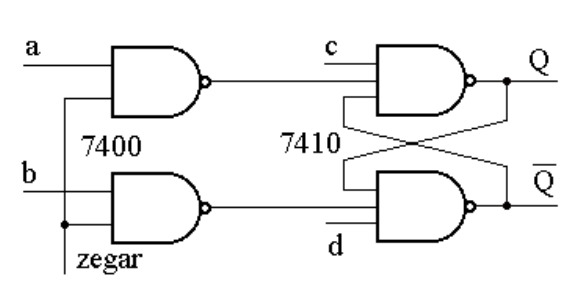
\includegraphics[width=7.5cm]{include/1/1.png}
    \caption{Schemat zbudowanego synchronicznego przerzutnika RS.}
\end{figure}
\clearpage
\section{}
Zamontowano układ scalony 7400 w gnieździe płytki UC-1 a następnie zbadano tablicę logiczną dla zawartych w nim bramek logicznych NAND.
Powyższe kroki powtórzono dla układu 7402 (NOR).
Ze względu na brak dostępności układ 7486 (XOR) nie został zbadany.

\begin{table}[H]
    \centering
    \begin{tabular}{c c | c c || c c}
        \hline
        \(U_A\)[V] & stan logiczny A & \(U_B\)[V] & stan logiczny B & \(U_Y\)[V] & stan logiczny Y
        \\ \hline\hline
        0          & 0               & 0          & 0               & 3.96       & 1               \\ \hline
        0          & 0               & 5.01       & 1               & 3.96       & 1               \\ \hline
        5.01       & 1               & 0          & 0               & 3.96       & 1               \\ \hline
        5.01       & 1               & 5.01       & 1               & 83m        & 0               \\ \hline
    \end{tabular}
    \caption{Wyniki badania bramki NAND w układzie 7400 (UCY7400), pomiary odpowiadają informacją zawartym w nocie katalogowej.}
\end{table}

\begin{table}[H]
    \centering
    \begin{tabular}{c c | c c || c c}
        \hline
        \(U_A\)[V] & stan logiczny A & \(U_B\)[V] & stan logiczny B & \(U_Y\)[V] & stan logiczny Y
        \\ \hline\hline
        0          & 0               & 0          & 0               & 3.96       & 1               \\ \hline
        0          & 0               & 5.01       & 1               & 162m       & 0               \\ \hline
        5.01       & 1               & 0          & 0               & 163m       & 0               \\ \hline
        5.01       & 1               & 5.01       & 1               & 161m       & 0               \\ \hline
    \end{tabular}
    \caption{Wyniki badania bramki NOR w układzie 7402 (74LS02), pomiary odpowiadają informacją zawartym w nocie katalogowej.}
\end{table}

\clearpage
\section{}
Zmontowano sumator o dwóch wejściach.
Zsumowano drgania sinusoidalne \(U_1\) i \(U_2\) z dwóch generatorów o zbliżonych częstotliwościach \(f_1 = 3\)kHz i \(f_2 = 3.2\)kHz.
Zmierzona częstotliwość powstałego w ten sposób przebiegu dudnień \(f_{dz} = 100.2\)Hz odpowiada wartości teoretycznej \(f_d = 100\)Hz wynikającej z obliczeń.

\begin{align}
    R_0    & = 19.77k\Omega                                             \\
    R_1    & = 1.99k\Omega                                              \\
    R_2    & = 2.01k\Omega                                              \\
    % 
    U_{wy} & = -\;R_0 \biggl( \frac{U_1}{R_1} + \frac{U_2}{R_2} \biggr)
    = -\biggl( 9.934\;U_1 + 9.836\;U_2 \biggr)                          \\
    f_d    & = \frac{|f_1 - f_2|}{2} = 100\text{Hz}
\end{align}

\begin{figure}[H]
    \centering
    \begin{circuitikz}[european]
        \draw (0, 0) node[op amp] (opamp) {};

        \draw (opamp.-) to[short, -*] ++(-1.5,0)
        coordinate (nNode);

        \draw (nNode) to[short, -] ++(0,0.5)
        to[R, l=$R_1$] ++(-2,0)
        node[anchor=east] {$U_{1}$};

        \draw (nNode) to[short, -] ++(0,-0.5)
        to[R, l=$R_2$] ++(-2,0)
        node[anchor=east] {$U_{2}$};

        \draw (opamp.-) to[short,*-] ++(0,1)
        coordinate (leftR)
        to[R, l=$R_0$] (leftR -| opamp.out)
        to[short,-*] (opamp.out)
        to[short,-*] ++(1,0)
        node[anchor=west] {$U_{wy}$};

        \draw (opamp.+)
        to[short,-] ++(0,-1)
        node[ground](GND){};
    \end{circuitikz}
    \caption{Schemat sumatora o dwóch wejściach}
\end{figure}

\begin{figure}[H]
    \centering
    \includegraphics[width=\textwidth]{include/3/1.png}
    \caption{Przebieg napięcia wyjściowego \(U_{wy}\)}
\end{figure}

\section{}
% Wyznaczyć średni czas propagacji impulsu przez bramkę mierząc okres drgań generatora zbudowanego z trzech bramek. Użyć do budowy generatora bramek serii podstawowej 7400. a potem bramek serii szybkiej 74S00. Porównaj wyniki.

Wyznaczono średni czas propagacji impulsu przez bramkę mierząc okres drgań generatora zbudowanego z trzech bramek NAND.
Do budowy generatora najpierw wykorzystano układ 7400, a następnie układ 74S00.
Uzyskane pomiary pomnożono przez \(\frac{1}{2*3}\), co dało czasy propagacji dla 7400 i 74S00 wynoszące odpowiednio \(10.38\)ns oraz \(3.5\)ns.
Czasy te zawierają się w zakresie dopuszczalnych wartości określonych w notach katalogowych układów.

\begin{figure}[H]
    \centering
    \begin{circuitikz}
        \draw
        (0, 0) node(gate1)[nand port] {}
        (2, 0) node(gate2)[nand port] {}
        (4, 0) node(gate3)[nand port] {};

        \draw
        (gate2.in 1) to[short,-] (gate2.in 2)
        (gate2.in 1 |- gate2.out) to[short,*-] (gate1.out);

        \draw
        (gate3.in 1) to[short,-] (gate3.in 2)
        (gate3.in 1 |- gate3.out) to[short,*-] (gate2.out);

        \draw
        (gate3.out) to[short,-*] ++(1, 0) coordinate (cen);

        \draw
        (gate1.in 1) to[short,-] (gate1.in 2)
        (gate1.in 1 |- gate1.out) to[short,*-] ++(-1, 0)
        to[short,-] ++(0, 1)
        to[short,-] (cen |-, 1)
        to[short,-] (cen);

        \draw
        (cen) to[short,-*] ++(1, 0)
        node[anchor=west] {$U_{wy}$};
    \end{circuitikz}
    \caption{Schemat układu generatora.}
\end{figure}

\begin{figure}[H]
    \centering
    \includegraphics[width=\textwidth]{include/4/1.png}
    \caption{Pomiar okresu drgań generatora zbudowanego przy pomocy układu 7400.}
\end{figure}

\begin{figure}[H]
    \centering
    \includegraphics[width=\textwidth]{include/4/2.png}
    \caption{Pomiar okresu drgań generatora zbudowanego przy pomocy układu 74S00.}
\end{figure}
\clearpage
\section{}
Zbudowano multiwibrator astabilny oraz zaobserwowano przebiegi impulsów na wyjściu układu oraz na kondensatorze.
Zmierzona częstotliwość drgań \(f_z=1.012\)kHz jest o \(11.3\%\) mniejsza od częstotliwości teoretycznej \(f\) wynikającej z obliczeń.
% Porównać zmierzoną wartości okresu drgań multiwibratora z wartością teoretyczną.

\begin{align}
    R_1 & = 109.5k\Omega \\
    R_2 & = 9.9k\Omega   \\
    R_3 & = 6.08k\Omega  \\
    C   & = 433nF
\end{align}
\begin{align}
    T = 2R_3C\:ln\frac{1+\gamma}{1-\gamma}
    \quad \text{gdzie} \quad \gamma =\frac{R_2}{R_1 + R_2}
\end{align}
\begin{align}
    \gamma & = 0.0829                                                                   \\
    T      & = 2 \cdot 6.08k\Omega \cdot 433nF \cdot ln \frac{0.9171}{1.0829} = 0.875ms \\
    f      & = \frac{1}{T} = 1.142kHz
\end{align}

\begin{figure}[H]
    \centering
    \begin{circuitikz}[european]
        \draw (0, 0) node[op amp] (opamp) {};

        \draw (opamp.-) to[short, -] ++(-2,0)
        coordinate (cap);

        \draw (cap) to[C, l=$C$] ++(0,-2)
        node[ground](GND){};

        \draw (cap)
        to[short, *-] ++(0,1.5)
        coordinate (p)
        to[R, l=$R_3$] (p -| opamp.out)
        to[short, -] (opamp.out);

        \draw (opamp.out)
        to[short,*-*] ++(2,0)
        node[anchor=west] {$U_{wy}$};

        \draw (opamp.out)
        to[R, l=$R_2$] ++(0,-2)
        coordinate (center);

        \draw (center)
        to[R, l=$R_2$] ++(0,-2)
        node[ground](GND){};

        \draw (opamp.+)
        to[short,-] (opamp.+ |- center)
        to[short,-*] (center);
    \end{circuitikz}
    \caption{Schemat multiwibratora astabilnego}
\end{figure}

\begin{figure}[H]
    \centering
    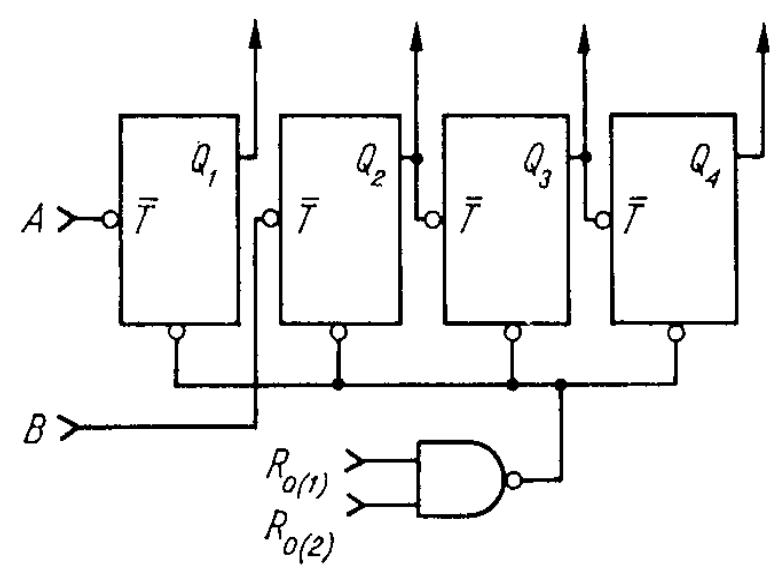
\includegraphics[width=\textwidth]{include/5/1.png}
    \caption{Przebiegi impulsów na wyjściu układu oraz na kondensatorze}
\end{figure}

\begin{figure}[H]
    \centering
    \includegraphics[width=\textwidth]{include/5/2.png}
    \caption{Napięcie na kondensatorze (Y) w funkcji napięcia na wyjściu układu (X)}
\end{figure}

\section{}
Zbudowano licznik modulo 10 modyfikując licznik modulo 16 z punktu 5.
Przy modyfikacji wykorzystano zawartą w układzie 7400 bramkę NAND, której celem jest śledzenie wyjścia licznika i podanie sygnału resetującego w momencie doliczenia do 10.

Stan wysoki wyjść \(Q_2\) i \(Q_4\) licznika (zakładając że zlicza on po kolei) jest warunkiem wystarczającym do stwierdzenia potrzeby resetu.
Jest to spowodowanie tym że wyjścia \(Q_2\) i \(Q_4\), są w stanie wysokim tylko gdy licznik doliczył do 10, 11, 14 lub 15.

Do wejść bramki NAND podłączono więc wejścia \(Q_2\) i \(Q_4\), natomiast do jej wyjścia podłączono \(R_0\) i \(R_1\).
Doliczenie do którejkolwiek z liczb 10, 11, 14 lub 15 powoduje pojawienie się zera logicznego na wejścia resetujące i zresetowanie licznika.

\section{}
Wykorzystując płytkę UC-1 zbudowano układ z dwóch rejestrów przesuwnych: 74164 i 74165.
Szeregowe wejście rejestru 74164 podłączono do impulsatora, wyjścia równoległe rejestru podłączono do wskaźników LED w celu śledzenia stanu rejestru.
Wyjścia równoległe układu 74164 podłączono również do wejść równoległych układu 74165, a jego wyjście szeregowe do próbnika stanów logicznych na płytce UC-1.
Utworzony w ten sposób szereg (impulsator, 74164, 74165, wskaźnik logiczny) testowano następująco.

Na wejście CLK rejestru 74164 podawano sygnał zegarowy, podając jednocześnie impulsy (z użyciem impulsatora) na wejście szeregowe.
Za pośrednictwem diod LED obserwowano stan rejestru przesuwnego: bity przesuwały się o jeden ilekroć układ wykrywał narastające zbocze sygnału zegarowego.
Najmłodszy bit odzwierciedlał stan impulsatora na wejściu szeregowym w momencie przesunięcia rejestru.

Następnie chcąc przetestować działanie układu 74165, ustalono stan na magistrali równoległej pomiędzy dwoma rejestrami impulsując na wejście 74164, przesuwając go odpowiednio.
W kolejnym kroku podano stan niski na wejście \(SH/\overline{LD}\) od 74165, co spowodowało zapis stanu ustalonego na magistrali równoległej do rejestru.
Zmieniono stan wejścia \(SH/\overline{LD}\) na wysoki, umożliwia to przesunięcie rejestru 74165 na skutek narastającego zbocza sygnału zegarowego, oraz jednoczesne uniewrażliwienie go na zmianę stanu magistrali.
Podawano następnie sygnał zegarowy obserwując jednocześnie stan wskaźnika logicznego na wyjściu szeregowym rejestru 74165.
Z kolejnymi narastającymi zboczami na wejściu CLK rejestr przesuwał się ustawiając stan wyjścia szeregowego na kolejne bity zapisane uprzednio na magistrali równoległej.

\end{document}